
X and Y are two independent random variables that can take the values 1, 2, 3, 4, 5, 6.
\begin{align}
    \Pr\brak{X=k}=\frac{1}{6}, 1\leq k \leq 6\\
    \Pr\brak{Y=k}=\frac{1}{6}, 1\leq k \leq 6
\end{align}
\begin{lemma}
The PMF of X+Y is given by\\
\begin{align}
\Pr\brak{X+Y=n}=
    \left\{
	        \begin{array}{ll}
		    \frac{n-1}{36}  & , 2 \leq n \leq 7 \smallskip\\
		    \frac{13-n}{36} & , 8 \leq n \leq 12
	        \end{array}
    \right.
\end{align}
\end{lemma}
\begin{proof}
Using convolution for discrete random variables,\\
$\Pr\brak{X+Y=n}$
\begin{align}
    =&\sum_{k=n-6}^{n-1} \Pr\brak{X=k,Y=n-k}, 1\leq k \leq 6
    \end{align}
    Since X and Y are independent,
\begin{align}
    =&\sum_{k=n-6}^{n-1} \Pr\brak{X=k}\times\Pr\brak{Y=n-k}, 1\leq k \leq 6
\end{align}
\begin{align}
    =&\sum_{k=n-6}^{n-1} \frac{1}{36}, 1\leq k \leq 6\\
    =&
    \left\{
	        \begin{array}{ll}
		    \frac{n-1}{36}  & , 2 \leq n \leq 7 \smallskip\\
		    \frac{13-n}{36} & , 8 \leq n \leq 12
	        \end{array}
    \right.\label{var/4/0.0.7}
\end{align}
\end{proof}
\begin{figure}[htb]
    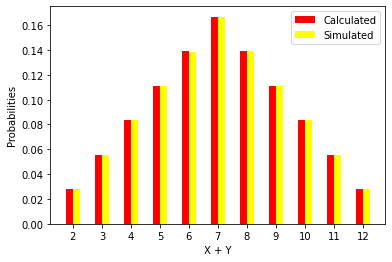
\includegraphics[width=\columnwidth]{variable/solutions/4/Figures/Assignment-4(1).png}
    \caption{Plot of PMF for X+Y}
\end{figure}
\begin{lemma}
The PMF of X-Y is given by\\
\begin{align}
    \Pr\brak{X-Y=n}
    =
    \left\{
	        \begin{array}{ll}
		    \frac{n+6}{36} & , -5 \leq n \leq 0 \smallskip\\
		    \frac{6-n}{36} & , 1  \leq n \leq 5
	        \end{array}
    \right.
\end{align}
\end{lemma}
\begin{proof}
Using convolution for discrete random variables,\\
$\Pr\brak{X-Y=n}$
\begin{align}
    =&\sum_{k=n+1}^{n+6} \Pr\brak{X=k,Y=k-n}, 1\leq k \leq 6
\end{align}
Since X and Y are independent,
\begin{align}
    =&\sum_{k=n+1}^{n+6} \Pr\brak{X=k}\times\Pr\brak{Y=k-n}, 1\leq k \leq 6
\end{align}
\begin{align}
    =&\sum_{k=n+1}^{n+6} \frac{1}{36}, 1\leq k \leq 6\\
    =&
    \left\{
	        \begin{array}{ll}
		    \frac{n+6}{36} & , -5 \leq n \leq 0 \smallskip\\
		    \frac{6-n}{36} & , 1  \leq n \leq 5
	        \end{array}
    \right.\label{var/4/0.0.12}
\end{align}
\end{proof}
\begin{figure}[htb]
    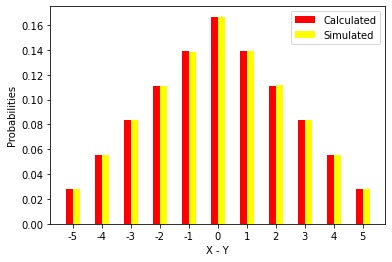
\includegraphics[width=\columnwidth]{variable/solutions/4/Figures/Assignment-4(2).png}
    \caption{Plot of PMF for X-Y}
\end{figure}
$E\brak{X+Y\:|\:(X-Y)^2=1}$
\begin{align}
    =&\sum\:n\times\Pr\brak{X+Y=n\:|\:(X-Y)^2=1}
\end{align}
\begin{align}
    =&\sum\:n\times\frac{\Pr\brak{X+Y=n,(X-Y)^2=1}}{\Pr\brak{(X-Y)^2=1}}
\end{align}
\begin{align}
    \begin{split}
        =\sum\:n\times\frac{\Pr\brak{X+Y=n,(X-Y)=1}}{\Pr\brak{(X-Y)=1}}
        \bigskip\\
        \times\Pr\brak{(X-Y)=1|(X-Y)^2=1}
        \bigskip\\
        +\sum\:n\times\frac{\Pr\brak{X+Y=n,(X-Y)=-1}}{\Pr\brak{(X-Y)=-1}}
        \bigskip\\
        \times\Pr\brak{(X-Y)=1\:|\:(X-Y)^2=1}
    \end{split}
\end{align}
\begin{align}
    \begin{split}
        =\:\frac{\Pr\brak{(X-Y)=1\:|\:(X-Y)^2=1}}{\Pr\brak{(X-Y)=1}}
        \bigskip\\
        \times\sum\:n\times\Pr\brak{X+Y=n,(X-Y)=1}
        \bigskip\\
        +\frac{\Pr\brak{(X-Y)=-1\:|\:(X-Y)^2=1}}{\Pr\brak{(X-Y)=-1}}
        \bigskip\\
        \times\sum\:n\times\Pr\brak{X+Y=n,(X-Y)=-1}\label{var/4/0.0.16}
    \end{split}
\end{align}
\newline\\\\
Using equations \eqref{var/4/0.0.7} and \eqref{var/4/0.0.12} in \eqref{var/4/0.0.16}\\
We get,\\
\newline
$E\brak{X+Y\:|\:(X-Y)^2=1}$
\begin{align}
    =&\:\brak{\frac{\frac{1}{2}}{\frac{5}{36}}}\times\brak{\frac{35}{36}}+\brak{\frac{\frac{1}{2}}{\frac{5}{36}}}\times\brak{\frac{35}{36}}\\
    =&\:7
\end{align}
